\documentclass[letterpaper,9pt,twocolumn,twoside,]{pinp}

%% Some pieces required from the pandoc template
\providecommand{\tightlist}{%
  \setlength{\itemsep}{0pt}\setlength{\parskip}{0pt}}

% Use the lineno option to display guide line numbers if required.
% Note that the use of elements such as single-column equations
% may affect the guide line number alignment.

\usepackage[T1]{fontenc}
\usepackage[utf8]{inputenc}

% pinp change: the geometry package layout settings need to be set here, not in pinp.cls
\geometry{layoutsize={0.95588\paperwidth,0.98864\paperheight},%
  layouthoffset=0.02206\paperwidth, layoutvoffset=0.00568\paperheight}

\definecolor{pinpblue}{HTML}{185FAF}  % imagecolorpicker on blue for new R logo
\definecolor{pnasbluetext}{RGB}{101,0,0} %



\title{Impacts of Transformation Techniques and Deep Learning Models on
Cell Images Classification Accuracy}

\author[]{Image02 - 510050786, 520181814, 510652339, 510401900,
520406670, 500469361}

  \affil[a]{The University of Sydney}

\setcounter{secnumdepth}{5}

% Please give the surname of the lead author for the running footer
\leadauthor{}

% Keywords are not mandatory, but authors are strongly encouraged to provide them. If provided, please include two to five keywords, separated by the pipe symbol, e.g:
 

\begin{abstract}

\end{abstract}

\dates{This version was compiled on \today} 


% initially we use doi so keep for backwards compatibility
% new name is doi_footer
\doifooter{\url{https://github.com/jiyu4399/DATA3888_Image_Group_2}}


\begin{document}

% Optional adjustment to line up main text (after abstract) of first page with line numbers, when using both lineno and twocolumn options.
% You should only change this length when you've finalised the article contents.
\verticaladjustment{-2pt}

\maketitle
\thispagestyle{firststyle}
\ifthenelse{\boolean{shortarticle}}{\ifthenelse{\boolean{singlecolumn}}{\abscontentformatted}{\abscontent}}{}

% If your first paragraph (i.e. with the \dropcap) contains a list environment (quote, quotation, theorem, definition, enumerate, itemize...), the line after the list may have some extra indentation. If this is the case, add \parshape=0 to the end of the list environment.


\hypertarget{executive-summary}{%
\section{Executive Summary}\label{executive-summary}}

Medical researchers often do not have supporting data to help classify
complex large-scale cell images, hence we aim to enhance classification
of cell images by gene expression cluster labels, without need for
supporting datasets.

The project found that data augmentation and masking techniques
significantly improves the classification accuracy. However, more
advanced and deeper networks capture the complex patterns among cell
images more efficiently thus having better predicting performance.

Within the report are key figures demonstrating our results with a bar
plot on basic CNN performance with data augmentation and masking
techniques, a comparative F1 score chart for ResNet18 versus basic CNN
across clusters, and an accuracy graph for VIT and transformers across
training epochs.

Actionable insights of the impact of data transformations and deep
learning models is in the creation of an interactive Shiny platform. The
application enables users, likely medical researchers, to upload cell
images and receive classifications based on selected models and
transformation techniques, translating complex data science processes
into actionable insights for users.

\hypertarget{introduction}{%
\section{Introduction}\label{introduction}}

The interpretation and classification of cell images based on gene
expression cluster labels play a crucial role in the fields of science
and medicine. Cells often exhibit complex phenotypes, such as variations
in shape, subcellular protein localization, and other characteristics.
The combination of these intricate phenotypic differences and diverse
biological responses makes deciphering biological processes increasingly
complex \citep{ShifatERabbi2019CellIC}. Therefore, traditional medical
research often struggles with image analysis and prediction due to
technical expertise limitations, which is a problem that tends to worsen
with increasing data volume and complexity \citep{panayides2020AI}. To
address this issue, the use of advanced computational techniques has
become increasingly popular. Computer analysis of cell images can
automatically classify cells, providing significant support in
scientific, technological, and medical applications. For instance, in
pathology, researchers are increasingly exploring methods to
automatically detect cancer through cell image classification
\citep{6fd805a257464dcc92460b6cf9dcee63}. The aim of this project,
therefore, is to investigate the impacts of different data processing
techniques and deep learning models on classification performance over
cell image data. Our primary focus is on leading medical and
biotechnological researchers who need to process large volumes of cell
imaging data, and are particularly interested in exploring cellular
localisation. To assist these researchers, we introduce a computer
vision scheme that accurately identifies cell identities and provides
detailed insights into the impact of various data transformations and
deep learning models on the classification results \textbf{(Figure 1)}.
This project thus seeks to help researchers gain a deeper understanding
of the potential drawbacks associated with their current data collection
and experimental design. By providing recommendations and insights, we
hope to refine the design and efficiency of cell classification
experiments, state-of-the-art methodologies from the data science field,
and achieve more accurate results. Given the complexity and
pervasiveness of cell images, we decided to focus on deep learning
methods, including convolutional neural networks (CNNs) and
Transformers, which have emerged as the leading end-to-end
classification system \citep{ShifatERabbi2019CellIC}. Our study also
includes various image augmentation techniques to enhance the
performance and accuracy of these models. Building on the key
findings,we developed an interactive platform - Shiny which will allow
users to get insights of models' performance by returning evaluation
metrics and detailed description about their selected combination of
model and data transformations techniques. The platform also allows
users to upload new cell images and select a specific set of model and
augmentation techniques to obtain predicted cluster IDs, along with
corresponding predicted probability. In creating a user-friendly
interface that translates complex data science processes into actionable
clear insights visually like Shiny could foster deeper understanding and
more effective application of cell image classification techniques.

\begin{figure}[h]
    \raggedright
    \includegraphics[width=0.45\textwidth]{Project workflow.png}
    \caption{Workflow}
    \label{fig:Workflow}
\end{figure}

\hypertarget{methodology}{%
\section{Methodology}\label{methodology}}

\hypertarget{data-acquisition}{%
\subsection{Data acquisition}\label{data-acquisition}}

The initial experimentation with the provided images using basic machine
learning techniques identified overfitting and low fitting efficiency as
significant issues (Appendix ). To address these, the project considered
an extended training input with transformation techniques (image contour
methods) and extended deep learning models. Therefore, the extended
image dataset, sourced from the 10X Genomics platform, includes
high-resolution cell images, cluster IDs, and cell boundary information
from a 10µm section of a C57BL/6 mouse from Charles River Laboratories.
The images are stored as lists, with each list representing a grayscale
image composed of an array of pixel intensity values. This dataset,
comprising 36,602 images across 28 clusters, was subsequently used for
further analysis.

\hypertarget{model-development}{%
\subsection{Model development}\label{model-development}}

Based on the reintroduced larger dataset and the problems identified
through experiments, it was evident that simple machine learning models
and the basic CNN model lacked the necessary complexity. Consequently,
our project narrowed its scope to focus solely on deep learning models.
ResNet18 and ResNet50 were considered initially, as these mainstream
classifiers learn the residual function of the reference layer input,
forming a network by stacking residual blocks, their architecture is
considered more suitable for optimisation. Beyond CNN models, another
main class investigated was Vision Transformers (ViT), which excel in
handling large datasets and offer more robust generalisation. The
overall deep learning models as shown:

\begin{itemize}
\tightlist
\item
  Basic CNN Model (CNN)
\item
  Resnet 18 (CNN)
\item
  Resnet 50 (CNN)
\item
  ViT (Transformer)
\end{itemize}

Specifically, the basic CNN model we constructed consists of two
convolutional layers with ReLU activation and 2x2 max pooling layers,
reducing the input dimensions from 50x50 to 12x12. ResNet18 comprises 18
layers including convolutional, batch normalisation, and identity
mapping layers, and ResNet50 consists of 50 layers with a more complex
architecture. Different from CNN models, the Vit model (Vit-base)
contains 12 layers.

\hypertarget{transformation-and-masking}{%
\subsection{Transformation and
Masking}\label{transformation-and-masking}}

In addition to efficient models, image augmentation has been proven as
an effective and efficient strategy to obtain satisfactory performance
with a limited dataset \citep{xu2023comprehensive}, which remains as a
prevalent obstacle in medical image analysis \citep{shorten2019survey}.
The project thus incorporates several image transformation and masking
techniques, including data normalisation and augmentation, with Gaussian
filters, Canny contour detection, Sobel edge detection.

Normalisation was applied to the pixel-based data by subtracting the
mean of pixel values and dividing by the standard deviation for each
image, projecting the pixel values within the predefined range of {[}0,
1{]} to ensure consistency within the training input. Image
augmentations such as random flipping and random rotation, have been
commonly utilised throughout many studies over the last decade for
various computer vision tasks such as image classification
\citep{xu2023comprehensive}, were also implemented with rotating angles
ranging from -50 to 50 degrees.

To further enhance model performance, Gaussian blur was implemented by
convolving each image with a Gaussian function to smooth the image and
reduce noise. This assigns a weight to each pixel based on its distance
from the centre, with the blur size set to (25, 25) to specify the
kernel size. The convolution operation calculates a weighted average of
the surrounding pixel values, reducing high-frequency noise.
Additionally, the Canny edge detection method was applied using
thresholds of 10 and 200 to detect a wide range of edges by identifying
intensity gradients. The final investigation focused on the Sobel edge
detector, which performs 2-D spatial gradient measurements on the image
to emphasise high spatial frequency regions corresponding to edges. To
evaluate the effectiveness of the two transformation, three masking
techniques, as well as to identify the most optimal combination with
different models, we established the Basic CNN model as our baseline.
This decision was made with consideration of the limited computational
resources available to the project team.

\begin{figure}[h]
    \raggedright
    \includegraphics[width=0.45\textwidth]{methodology.png}
    \caption{Methodology}
    \label{fig:methodology}
\end{figure}

\hypertarget{training-and-validation}{%
\subsection{Training and Validation}\label{training-and-validation}}

The training and validation process began by experimenting with
different combinations of transformation techniques on the dataset,
which was initially split into 80\% training and 20\% testing sets. For
all of the CNN models, based on 4-fold cross-validation, the training
set was further divided into four folds, each containing 20\% of the
data, and models were trained using these folds. Considering the
limitation of computational resources, the ViT model, along with the
optimal CNN model, was trained and validated with a single validation
set.

During training, instances of overfitting were observed, which were
addressed by adding dropout layers to each model. Additionally, the
performance of three optimizers---SGD, BGD, and ADAM---was compared,
where SGD exhibited noticeable fluctuations, BGD had slow convergence,
and ADAM, being relatively robust, was ultimately chosen for all models.
Upon completing the training process, the final model's performance was
evaluated using the untouched testing set.

\hypertarget{evaluation-strategy}{%
\subsection{Evaluation strategy}\label{evaluation-strategy}}

Our evaluation strategies to gauge model performance measured both
per-cluster and overall levels. Accuracy serves as the primary indicator
of model success, while precision and recall provide more nuanced
insights into the model's predictive capabilities, particularly in class
imbalances. Precision indicates the proportion of true positive
predictions out of all positive predictions made by the model, while
recall measures the proportion of true positive cases detected out of
all actual positive cases. Generally, precision and recall are inversely
related: a more conservative model might have higher precision but lower
recall, and vice versa.

To address this, we calculated the F1 score, which balances both
precision and recall to provide a single metric that considers both
false positives and false negatives. However, we also report precision
and recall separately to allow for more specific evaluation scenarios.
Furthermore, the confusion matrix further measures model performance by
revealing possible patterns of misclassification. To ensure scalability
and feasibility for real-world applications, the models are also
evaluated in terms of running time and memory usage.

\hypertarget{result}{%
\section{Result}\label{result}}

\hypertarget{convolutional-neural-networks-cnns}{%
\subsection{Convolutional Neural Networks
(CNNs)}\label{convolutional-neural-networks-cnns}}

\hypertarget{basic-cnn-model}{%
\subsubsection{Basic CNN model}\label{basic-cnn-model}}

Applying image augmentation techniques yields noticeable improvements in
the performance of the basic CNN model. Specifically, using the
transformed dataset increases 2.6\% of accuracy, 3\% of precision, and 1
of F1 score than the original one \textbf{(Figure 3)}. Normalisation
also accounted for most of the results, noticeably doubling the
precision. Given the fact that normalisation reduces the differences
between the variation range of the different variables, error gradually
decreases \citep{sola1997importance} which improves both convergence and
generalisation of the network \citep{shao2020normalization}.

Image augmentation techniques (random rotation and random flip), except
for increasing the accuracy 0.9\%, has no impact on the precision and
even decreases the F1 score by 1 \textbf{(Figure 3)}. As these cells in
medical images can appear in many variations, these geometric
transformations can introduce variability into the model by changing the
perspectives of objects within images mitigating the overfitting issue
encountered initially \citep{xu2023comprehensive}. However, as both the
angle of rotation and axis of flipping directly affect the preservation
label identity and variations in the dataset
\citep{xu2023comprehensive}, the unfavourable outcome might indicate
that the chosen magnitude of these operations within this project is not
the most optimal one.

All the masking techniques, meanwhile, appear to contribute little to
the improvement of model performance. They even worsen the model's
accuracy by 0.5 - 0.7\% \textbf{(Figure 3)}. Although the edge detection
and blur type identification techniques have been proven to have
remarkable performance on deep learning models
\citep[\citet{guo2021non}]{wang2017blur}, the simple architecture of the
basic CNN causes its limited capacity and sensitivity to input
variations of architecture, which might lead to less capability of
benefiting from such complex image preprocessing techniques like
masking. The lack of the improvement could indicate that the basic CNN
model's architecture is not sophisticated enough to capitalise on the
increased variability without additional modification
\citep{tuggener2022enough}.

\begin{figure}[h]

{\centering 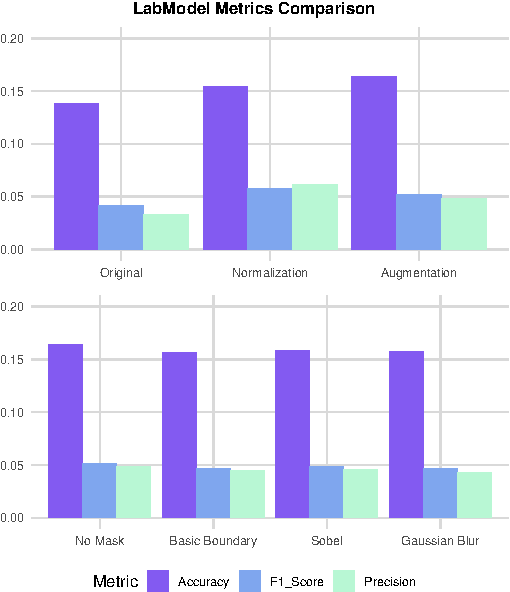
\includegraphics{Image02_final_report_files/figure-latex/unnamed-chunk-2-1} 

}

\caption{Basic CNN model under different data transformation and masking techniques}\label{fig:unnamed-chunk-2}
\end{figure}

\hypertarget{advanced-cnn-models-resnet-models}{%
\subsubsection{Advanced CNN models (ResNet
models)}\label{advanced-cnn-models-resnet-models}}

Applying masking techniques on more advanced CNN models shows contrary
results, significantly improving the models' accuracy. Specifically,
including the cell boundary increases the accuracy by 3.3\% on ResNet18
and 2.2\% on ResNet50. Using sobel edge adds 4.3\% more on the accuracy
of ResNet18, and 0.4\% for ResNet50. Gaussian blur, which is also the
masking technique with best performance on advanced CNNs, better the
ResNet18's accuracy by 6.4\% and ResNet50 by 5.16\% \textbf{(Figure 7)}.
Given the deeply sophisticated architectures, these two networks appear
to gain significant advantages from these advanced image preprocessing
methods: masking to better their performance.

\hypertarget{overall-cnn-models}{%
\subsubsection{Overall CNN models}\label{overall-cnn-models}}

Comparing the performance of three CNN models over 30 epochs based on
the optimal combination (\textbf{Figure 8}), the basic CNN model
achieved a validation accuracy of 15\%, with both training and
validation curves remaining smooth. ResNet18 reached a validation
accuracy of 17\%, stabilizing after initial fluctuations, while ResNet50
achieved approximately 14.5\%. None of the models exhibited overfitting,
indicating the effectiveness of our preprocessing methods.

Further comparing the F1 scores at the per-cluster level, the ResNet18
model demonstrates superior performance with an average F1 score of
0.09, better than the average F1 score for ResNet50 (0.07) and basic CNN
model (0.05) \textbf{(Figure 9)}. This indicates that, on average, the
ResNet18 balances precision and recall better than others. Specifically
\textbf{(Figure 4)}, for Cluster 6, ResNet18 achieves an F1 score of
0.45, which matches the performance of the basic CNN. But ResNet18 also
outperforms the basic CNN in several other clusters (clusters 2 and 3),
by achieving higher F1 scores, indicating its robustness and better
generalization capabilities compared to the basic CNN.

Overall, the ResNes18 would be the best model, and as ResNet50 and basic
CNN have similar accuracies but better F1-score, we suggest ResNet50
still outperforms basic CNN.

The good performance of ResNet18 can be attributed to its more complex
architecture, which includes additional convolutional and pooling
operations \citep{article}, allowing it to capture more intricate
features compared to the basic CNN model.

Interestingly, ResNet50 did not outperform the basic CNN with its
accuracy but the F1-score, in the F1 distribution, while the basic CNN
model shows a higher F1 score for certain clusters, both ResNet provide
more comprehensive predictions across all clusters. We believed it could
be attributed to the observed imbalance in the data, where the basic CNN
model's tendency to over-predict certain clusters likely contributed to
its seemingly better performance in those specific cases. In addition to
this, as the ResNet50 is more complex with the architecture, the lack of
performance in ResNet50 compared to ResNet18 might still be due to the
model's tendency to over-predict certain clusters for ResNet18. The
imbalance issue also leads to its comparable or even lower performance.

\begin{figure}[h]

{\centering 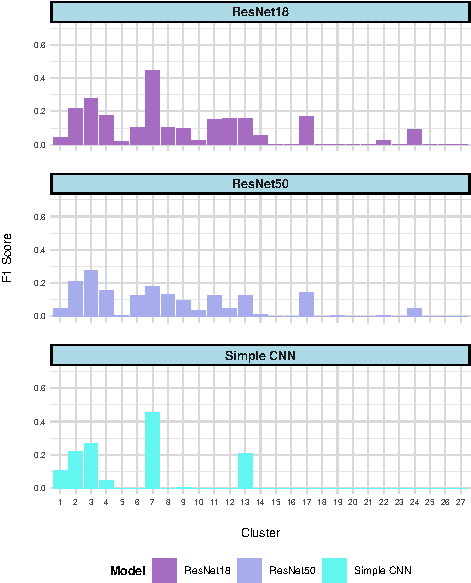
\includegraphics{Image02_final_report_files/figure-latex/unnamed-chunk-3-1} 

}

\caption{F1 Scores by Cluster for all Models}\label{fig:unnamed-chunk-3}
\end{figure}

\hypertarget{transformers-vit}{%
\subsection{Transformers (ViT)}\label{transformers-vit}}

Under the single validation training \textbf{(Figure 5)}, the accuracy
of the ViT model increased steadily and continued to grow, while the
validation accuracy began to stabilise at around 17.5\% after 10 epochs
(Figure). In the latter half of the training, we observed signs of
overfitting, but the validation curve did not decline significantly, it
was considered as a ``good'' overfitting.

Comparing the single validation training of the best CNN model
(ResNet18) \textbf{(Figure 5)}, ViT outperformed the CNN by
approximately 4\% in accuracy. Additionally, ViT made predictions on
more clusters (wider prediction) and exhibited higher precision and
recall both for each cluster and overall \textbf{(Figure 10)}.
Therefore, it could be concluded that the ViT model simultaneously
satisfies a wide range of predictions and recalls, and demonstrates
better performance. This improved performance can be attributed to the
generalisation capabilities, the ability to capture global context,
combined with its extensive pretraining on large datasets.

\begin{figure}[h]

{\centering 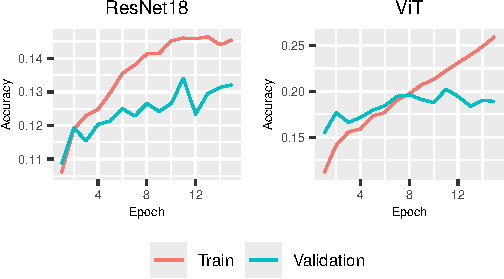
\includegraphics{Image02_final_report_files/figure-latex/unnamed-chunk-5-1} 

}

\caption{Train and validation accuracy between ViT and ResNet18}\label{fig:unnamed-chunk-5}
\end{figure}

\hypertarget{shiny}{%
\subsection{Shiny}\label{shiny}}

Key findings are then visualized and presented using an interactive
\href{https://gitparth12.shinyapps.io/data3888_imaging_021/}{platform
Shiny}, which enables a more engaging and informative approach to the
end-users. The app has three main functions \textbf{(Figure 6)},
including:

\begin{enumerate}
\def\labelenumi{\arabic{enumi}.}
\item
  Providing insights of CNNs performance (accuracy, precision, F1 score,
  etc.). Considering that the dataset has a huge class imbalance
  problem, Shiny also displays models' performance both overall and
  across 28 clusters.
\item
  Providing insights of the Transformers (ViT), with detailed comparison
  with the best model from CNN class: ResNet18.
\item
  Predicting clusterID and corresponding predicted probability of cell
  image uploaded by users, using selected combination of model and data
  transformation, masking techniques.
\end{enumerate}

\hypertarget{discussion-and-conclusion}{%
\subsection{Discussion and Conclusion}\label{discussion-and-conclusion}}

The project findings highlight the importance of selecting appropriate
data transformations and model architectures for the task of cell image
classification. Normalisation was an universally beneficial
preprocessing step, while the effectiveness of image augmentation and
masking techniques varied depending on model complexity. The basic CNN
model's limitations were highlighted by its inability to benefit from
more complex preprocessing methods, whereas advanced CNN models
demonstrated significant improvements when these techniques were
applied. Overall, ViT appears as the best model with highest prediction
performance.

However, it is critical to acknowledge that the success of deep learning
in vision depends on three factors: high capacity models, computational
power, and availability of large-scale labelled data
\citep{sun2017revisiting}. The project's scope and methodology still has
several limitations. Specifically, the small dataset size constrained
the complexity of the models that could be trained, as more
sophisticated models require larger datasets to be effective. The
significant imbalance issue across clusters might also potentially
introduce certain biases into the models. Additionally, the vague nature
of the cluster labels posed a challenge for model interpretability,
making it difficult to understand the basis for the model's predictions.
Other shortcomings, such as the low model complexity due to limited
computing resources and the lack of interpretability, highlight areas
for future work to improve the methodology approach.

Therefore, future work can leverage more data from under-represented
classes to address the class imbalance issues such as a dataset
including the full brain to provide a richer and more varied set of
images for analysis. More advanced and deeper network architectures
should also be considered for better prediction given the complexity of
medical visuals such as cell images. Given that ViT outperforms all CNNs
being considered, more networks from this class can be trained to
investigate the efficiency of Transformers in medical image analysis.
Additionally, the application of cross-validation (CV) across all models
would ensure a more robust evaluation of their performance.

\section*{Group Contribution}

\textbf{Parth Bhargava (510401900):} Converted the Imaging lab set up
code from R to Python. Trained some basic CNNs (with J). Worked on
Shiny's backend: matched the project's result with the UI's design of
models' performance, Image prediction tab. Generated some plots for the
final report. Structurised and arranged the group's GitHub repository.

\textbf{MiaoMiao Chen (520181814):} Initial exploration with three
masking techniques, the initial ResNet50 model, the basic machine
learning models with Hazel, workflow figure, the Methodology figures
(with Hazel), part of Shiny design, part of script, part of presentation
slides, responsible for the meeting minutes submission, report's
methodology, second half of report's results,report formatting in r.

\textbf{Ethan Chang (520406670):} I took notes during workshops and
consultations, refined and created slides based on tutor feedback,
helped with initial lab model transformations, and improved the
presentation script for clarity and flow, ensuring it stayed within the
time limit. I created the report abstract, co-wrote the executive
summary and improved phrasing.

\textbf{Hazel Nguyen (510652339):} Fitting KNN, Random Forest (with
Miaomiao). Two main figures: Workflow \& Methodology (with Miaomiao).
Part of the Shiny's UI design. Presentation slides (including recorded
video of Shiny) and part of the script. Report template and rendering
using R's pinp, first half of the report's result, part of the
discussion and conclusion.

\textbf{Evan Nguyen (500469361): }I was responsible for writing and
editing the report and the presentation script. Additionally I also
helped with initial data exploration and assisted with looking into some
basic transformation techniques for cells.

\textbf{Jiacheng Yu (510050786):} I primarily managed the architecture
and most of the fine-tuning and training process for deep learning
models, concluded save and visualization. Moreover, I explored the shiny
app for Python. and built the code architecture for the whole project.
Also, I drew about half of the diagrams in the final report.

\newpage

\hypertarget{github-and-shiny-link}{%
\section{Github and Shiny Link}\label{github-and-shiny-link}}

\url{https://github.com/jiyu4399/DATA3888_Image_Group_2}

\url{https://gitparth12.shinyapps.io/data3888_imaging_021/}

\hypertarget{appendix}{%
\section{Appendix}\label{appendix}}

\begin{figure}[h]
    \raggedright
    \includegraphics[width=0.4\textwidth]{shiny.png}
    \caption{Shiny}
    \label{fig:Shiny}
\end{figure}

\begin{figure}[h]

{\centering 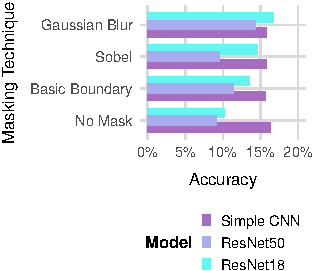
\includegraphics{Image02_final_report_files/figure-latex/unnamed-chunk-6-1} 

}

\caption{Models accuracy under different masking techniques}\label{fig:unnamed-chunk-6}
\end{figure}

\begin{figure}[h]

{\centering 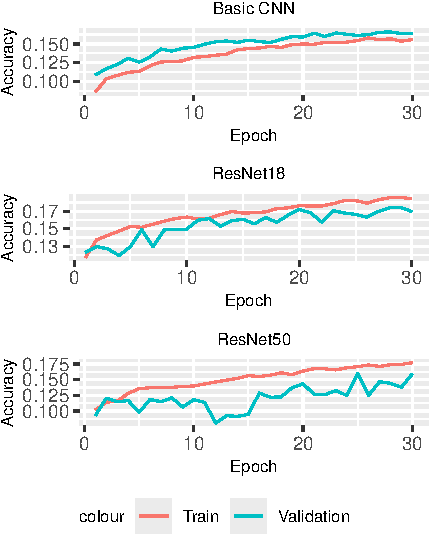
\includegraphics{Image02_final_report_files/figure-latex/unnamed-chunk-7-1} 

}

\caption{Train and validation accuracy for all models}\label{fig:unnamed-chunk-7}
\end{figure}

\begin{figure}[h]

{\centering 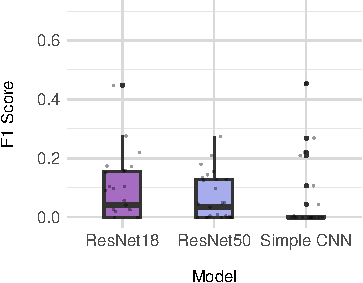
\includegraphics{Image02_final_report_files/figure-latex/unnamed-chunk-8-1} 

}

\caption{Average F1 Score Distribution for all models}\label{fig:unnamed-chunk-8}
\end{figure}

\vspace{10 cm}

.

\begin{figure}[h]

{\centering 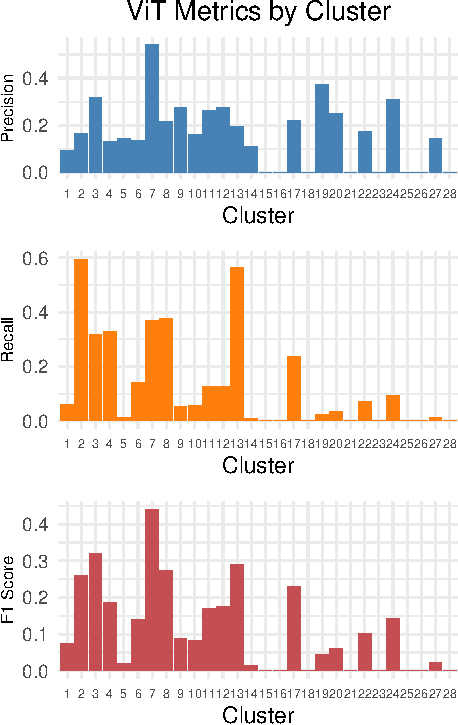
\includegraphics{Image02_final_report_files/figure-latex/unnamed-chunk-9-1} 

}

\caption{F1 score per cluster for Vit}\label{fig:unnamed-chunk-9}
\end{figure}

\vspace{10 cm}

.

\begin{figure}[h]

{\centering 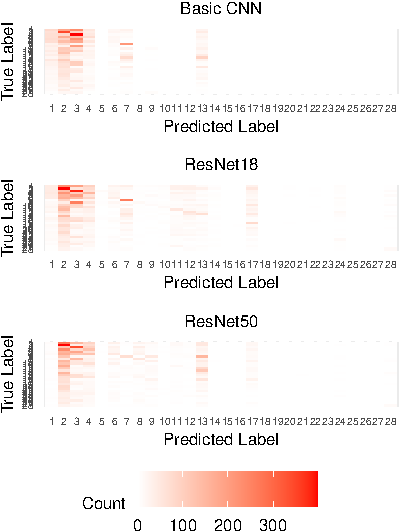
\includegraphics{Image02_final_report_files/figure-latex/unnamed-chunk-10-1} 

}

\caption{confusion matrix}\label{fig:unnamed-chunk-10}
\end{figure}

\newpage

%\showmatmethods


\bibliography{report.bib}
\bibliographystyle{jss}



\end{document}
